\documentclass{article}

\title{Simulating and Reconstructing X-Ray CT Projections}
\author{Reece Garthwaite}
\date{}

\usepackage{graphicx}
\usepackage{amsmath}

\begin{document}
\maketitle

\begin{abstract}
I have chosen to simulate x-ray transmission through a digital phantom, using energy dependent attenuation to generate sinograms that I then reconstruct using simple back projection. I used NIST data to model bone and soft tissue with energy dependent attenuation coefficients.
\end{abstract}

\section{Introduction}
Computed tomography scans are a form of medical imagery that uses X-rays to  create images of the body. CT scans reconstruct cross sectional images of the body from multiple projections of X-ray attenuation through an object. In this project, I go through a large amount of the process of X-ray imaging: from simulating the incident X-rays using the python software toolkit spekpy, to simulating the x-ray attenuation and forming a spectogram, which I then use simple back projection to reconstruct the X-ray image.

\section{Methods}

\subsection{Background Physics}
\subsubsection{X-ray generation}
X-rays are produced when high kinetic energy electrons are accelerated towards a positive anode in a x-ray tube. Tungsten is a common choice for the anode (due to its high melting point and high atomic number). Electrons come close to nuclei of the target, causing a deceleration and change in direction, converting kinetic energy into a spectrum of electromagnetic radiation. Incident electrons can ionise the material, removing an electron from the anode. As the electron orbit vacancy gets filled by a orbital shell electron in a further out shell a photon is emitted. As orbital energies and their differences are unique in atoms, this leads to what we call "characteristic radiation".
\cite{Tafti}

\begin{figure}
  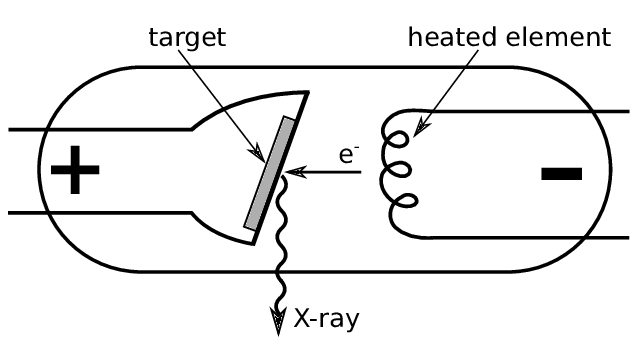
\includegraphics[width=\linewidth]{xray_tube.png}
  \caption{A X-ray tube}
  \label{fig:X-ray tube}
\end{figure}
Figure \ref{fig:X-ray tube} shows a diagram of a X-ray tube. \cite{Mason}

\subsubsection{Attenuation of X-rays}
As X-rays pass through matter, they are attenuated according to the Beer-Lambert law: 
\begin{equation} \label{bl}
I(E) = I_0 \cdot e^{-\mu(E) x}
\end{equation}

Where:
\begin{itemize}
  \item I = transmitted intensity of radiation after passing through the material
  \item $I_0$ : Initial intensity
  \item $\mu$ : Linear attenuation coefficient
  \item $x$ : Thickness of material
\end{itemize}

I have included  $\mu$ to be energy dependent as this is what is observed in experiments, and allows us to look for an interesting phenomenon known as beam hardening. I calculate $\mu$ using:
\begin{equation} \label{linearatt}
\mu(E) = \left(\frac{\mu}{\rho}\right) \cdot \rho
\end{equation}
using mass attenuation data from NIST and known material densities.

\bibliography{References}
\bibliographystyle{ieeetr}
\end{document}
